\chapter{Introduction}\label{ch:introduction}
The basic approach of our project, just like any other based on embedded systems (\textit{microcontrollers}) largely depends on three main questions: 
\begin{itemize}
	\item Which microcontroller board would be appropriate?
	\item What \textit{sensor}(s) should be used to fulfill the goals of the project? 
	\item What actuators might be needed for introducing mechanical action, if needed? 
 
\end{itemize}

We had a literature survey through the internet about deciding the components needed for our project. This included studying in detail, several project ideas and instructions posted on blogs and YouTube.\\
We selected the following major components for having a \textsl{minimal}, \textsl{cost effective} and \textsl{efficient} apparatus that could do the job for us:
\begin{itemize}
	\item \textit{Microcontroller Board} - \arduinouno{}
	\item \textit{Sensor} - \hcsr{} \ultrasonic{}
	\item \textit{Actuator} - \servo{} Motor

\end{itemize}
The next few sections will explain the basis of selection of hardware for this project.

% r~\ref{ch:ch2label}.
\clearpage
\section{The \arduinouno}
\begin{figure}[H]
	\centering
	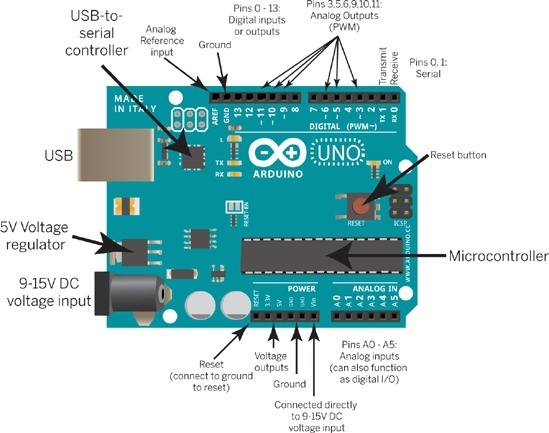
\includegraphics[width=0.5\textwidth]{../Files/arduino_parts.jpeg}
	\caption{The Arduino UNO}  \label{fig:Arduino}
\end{figure}
Arduino is an open source electronics platform for fast prototyping of projects for users with minimal knowledge or experience in electronics and programming. We have used the \arduinouno, the most widely used variant of the Arduino.\\
Technically, Arduino Uno is a microcontroller board based on the 8-bit ATMega328P microcontroller. With 14 digital
input/output pins (including 6 PWM outputs), 6 analog inputs, a 16 MHz ceramic resonator, a USB connection, a power jack, an ICSP header, and a reset button, it has everything needed to support the microcontroller; we simply have to connect it to a computer with a USB cable or power it with a AC-to-DC adapter or battery to get started.\\
Arduino also comes with the Arduino IDE, in which we can write code and upload to the Arduino. The programming language used for an Arduino, called the Arduino Programming language, is very similar to C/C++ except that we can use inbuilt functions of the Arduino libraries which keep the code very simple and short.

\subsection{Why Arduino?}
We had the following reasons strongly backing our decision to choose the \arduinouno :
\paragraph{\textit{Support -}}
 Thanks to its simple and accessible user experience, Arduino has been used in thousands of different projects and applications. The Arduino software is easy-to-use for beginners, yet flexible enough for advanced users. It runs on Mac, Windows, and Linux.\\
 This has enabled a very large support base for Arduino, more than any other microcontroller board ever released in the market. Every problem/bug/question that we ever had throughout the course of this project was promptly answered by questions in online forums, as there was a very high probability that scores of people had already posted the same question and the issue was resolved by other experienced users.
 \paragraph{\textit{Cost Effective -}}
 The Arduino UNO, its basic variant that every beginner to embedded systems usually starts with, is available for less than \$25. Being an open source hardware and due to its simplicity, it is easily and widely replicable, which is also responsible for the growth of such a large community as mentioned in the earlier reason.
 \paragraph{\textit{Features -}} 
 \begin{table}
 \centering
 \begin{tabular}{|l|l|}
 	\hline
 	Microcontroller &ATmega328P(8-bit)\\
 	\hline
 	Operating Voltage &(DC)5V\\
 	\hline
 	Input Voltage  &(recommended) 7-12V; (limits) 6-20V\\
 	\hline
 	Digital I/O Pins &14 (of which 6 provide PWM output)\\
 	\hline
 	Analog Input Pins &6\\
 	\hline
 	DC Current per I/O Pin &40 mA\\
 	\hline
 	DC Current for 3.3V Pin &50 mA\\
 	\hline
 	Flash Memory &32 KB (ATmega328) of which 0.5 KB used by bootloader\\
 	\hline
 	SRAM &2 KB (ATmega328)\\
 	\hline
 	EEPROM &1 KB (ATmega328)\\
 	\hline
 	Clock Speed &16 MHz\\
 	\hline
 	Need of External Programmer &NO\\
 	\hline
 	Built-in LED &pin13\\
 	\hline
 	Length &68.6 mm\\
 	\hline
 	Width &53.4 mm\\
 	\hline
 	Weight &25 g\\
 	\hline
  \end{tabular}
  \caption{Features of Arduino UNO}
  \label{tab:FeaturesArduino}
\end{table}
 It is generally observed that the computing power and inbuilt memory of the Arduino easily supports a wide variety of circuits with multiple components along with continuous serial communication with another device/computer. Compared to the system configuration of the board, our project would require fairly low amount of resources. \vspace{0.1cm} \linebreak 
 The no. of GPIO pins on the UNO is more than sufficient considering the need for the circuitry in our project, as we shall see when we look at the pinouts of the servo motor and the sensor - the only two other devices being used in the project. \vspace{0.1cm} \linebreak
 One important advantage of using the UNO is that unlike most previous programmable circuit boards, the \textit{Arduino UNO does not need a separate piece of hardware (called a programmer) in order to load new code onto the board} – we can simply use a USB cable. The ATmega328 on the Arduino/Genuino Uno comes preprogrammed with a \textit{bootloader} that allows us to upload new code to it without the use of an external hardware programmer. \vspace{0.1cm} \linebreak
 Moreover, the components we have used work under the same operating voltage and current conditions as an arduino, especially considering the fact that such components are nowadays sold with their compatibility with arduino in mind.\\
 
 Considering the above factors, we found Arduino UNO to be the most appropriate microcontroller board to work with for this project.\\
 
\subsection{Operation of Arduino}
Once a program written for an \textit{Arduino}, called a "\textit{Sketch}" is uploaded to the board via the Arduino IDE, the Arduino environment performs some small transformations to make sure that the code is correct C/C++. It then gets passed to a compiler (\textit{avr-gcc}), which turns the human readable code into machine readable instructions (\textit{object }files). Then, the code gets combined with (\textit{linked} against) the standard Arduino libraries that provide basic functions like \emph{digitalWrite()} or \emph{Serial.print()}. The result is a single Intel \emph{hex} file, which contains the specific bytes that need to be written to the program(\textit{flash}) memory of the chip on the Arduino board. This file is then uploaded to the board: transmitted over the USB or serial connection via the bootloader already on the chip or with external programming hardware.

\section{The \hcsr{} \ultrasonic{}}
\begin{figure}[H]
	\centering
	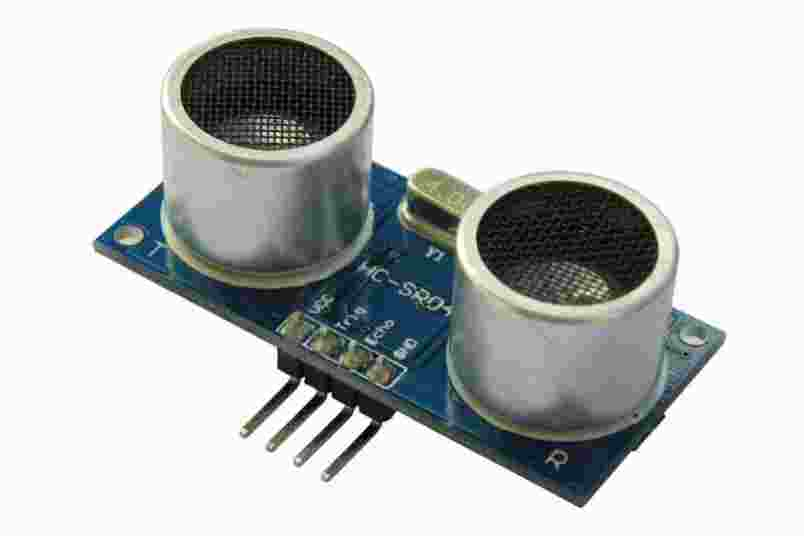
\includegraphics[width=0.5\textwidth]{../Files/HCSR04.jpg}
	\caption{HC-SR04 Ultrasonic sensor}  \label{fig:HCSR}
\end{figure}
The HC-SR04 ultrasonic sensor uses sonar to determine distance to an object like bats or dolphins do. It offers non-contact range detection from 2cm to 400 cm or 1” to 13 feet. It's operation is not affected by sunlight or black material like sharp rangefinders are (although acoustically soft materials like cloth can be difficult to detect). It comes complete with ultrasonic transmitter and receiver module.\\
The human ear can only detect sounds betwen 20Hz-20kHz. The sound waves beyond 20kHz are called ultrasonic waves or ultrasound.\\
The principle of ultrasonic distance measurement uses the velocity of ultrasonic waves spreading in air, measuring the time from launch to reflection when it encounters an obstacle. We then calculate the distance between the transmitter and the obstacle according to the time and the velocity. Thus, the principle of ultrasonic distance measurement is the same as with a radar.

\subsection{Features}
\begin{table}
	\centering
	\begin{tabular}{|l|l|}
		\hline
		Electrical Parameters &HC-SR04 Ultrasonic Module\\
		\hline
		Operating Voltage &(DC)5V(4.5-5.5V)\\
		\hline
		Quiescent Current(inactivity)  &2mA(1.5-2.5mA)\\
		\hline
		Working Current  &15mA(10-20mA)\\
		\hline
		Operating Frequency &40KHZ(ultrasonic)\\
		\hline
		Farthest Range &4m\\
		\hline
		Nearest Range &2cm\\
		\hline
		Resolution &0.3cm\\
		\hline
		Measuring Angle &15 Degrees\\
		\hline
		Input Trigger Signal &10us TTL pulse\\
		\hline
		Output Echo Signal &Output TTL level signal, proportional
		with range\\
		\hline
		Dimensions &45*20*15mm\\
		\hline

	\end{tabular}
	\caption{Features of HC-SR04}
	\label{tab:FeaturesHCSR}
\end{table}
The reason to choose this sensor was due to its reasonable range of taking measurements of the presence of an object for very less cost and electrical/computational resources. It's features are given in Table \ref{tab:FeaturesHCSR}.
\subsubsection{Note - Use of only stationary objects}
Since the sensor considers the distance to an obstacle that reflects the ultrasonic wave, we cannot use it to make trustworthy measurements of the position of \emph{moving} objects. This is majorly due to the fact that this sensor works on the principle of transmitting a set of pulses and recieving their reflection, before transmitting again, as we shall see later. Hence, there is no way that we can continuously track the position of an object with such a sensor. As far as we know, that can only be done by some type of a \textit{camera}, which would've introduced the concepts of computer vision and taken us beyond the scope and costs of the current project.

\subsection{HC-SR04 : Pin Definitions}
\begin{itemize}
	\item Vcc  - 5V Power Supply
	\item Trig - Trigger Pin (Input)
	\item Echo - Receive Pin (Output)
	\item GND  - Power Ground
\end{itemize}
The \emph{Trig} and \emph{Echo} pins are used for tranmission and reception of ultrasonic waves, respectively. 

\subsection{Operation of the HC-SR04}
\begin{figure}[H]
	\centering
	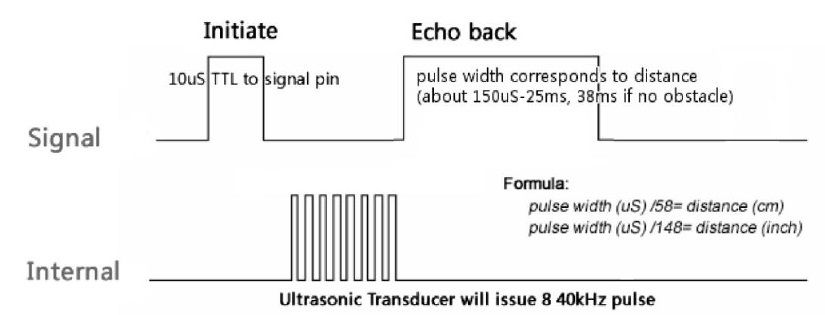
\includegraphics[width=0.5\textwidth]{../Files/hcsr_timing.png}
	\caption{Timing Diagram of HC-SR04 Ultrasonic sensor}  \label{fig:HCSRTiming}
\end{figure}
The timing diagram of HC-SR04 is shown in Figure \ref{fig:HCSRTiming}. To start measurement, Trig of SR04 must receive a HIGH pulse (5V) for at least 10us, which will initiate the sensor to transmit 8 cycles of ultrasonic burst at 40kHz. It then waits for the reflected ultrasonic wave. When the sensor detects the ultrasonic wave through the receiver, it will set the Echo pin to HIGH (5V), for as long as it detects an incoming ultrasonic pulse at the receiver.
\subsubsection{Calculation of distance}
The delay between tranmission and reception of the final pulse (i.e., between when the Trig pin is set back to LOW and when the Echo pin turns HIGH) is a time period proportional to the distance travelled by it. To obtain the distance, we start a counter the moment the Trig pin is set to LOW which keeps counting till the microcontroller detects a HIGH pulse at the Echo pin.
Time = Width of pulse, in uS (micro second).
\begin{itemize}
	\item Distance in centimeters = Time / 58
	\item Distance in inches = Time / 148
\end{itemize}
as mentioned in its datasheet. We can also utilize the speed of sound, which is 340m/s in a generic case.\\
This entire process can be translated into the Arduino code as shown in example \ref{ex:duration_example}.
\begin{example}{Arduino Code for calcuating distance from HC-SR04 sensor}
\label{ex:duration_example}
\begin{mdframed}[backgroundcolor=light-gray, roundcorner=10pt,leftmargin=1, rightmargin=1, innerleftmargin=15, innertopmargin=15,innerbottommargin=15, outerlinewidth=1, linecolor=light-gray]
	\begin{lstlisting}[language = C]
	/* Function for calculating the distance measured by the Ultrasonic sensor*/
	float calculateDistance(){ 
	unsigned long T1 = micros();
	digitalWrite(trigPin, LOW); // trigPin needs a fresh LOW pulse before sending a HIGH pulse that can be detected from echoPin
	delayMicroseconds(2);//DELAY #2:time for which low trig pulse is maintained before making it high
	digitalWrite(trigPin, HIGH); 
	delayMicroseconds(10);//DELAY #3:Sets the trigPin on HIGH state for 10 micro seconds
	digitalWrite(trigPin, LOW);
	duration = pulseIn(echoPin, HIGH); // Reads the echoPin, returns the sound wave travel time in microseconds
	distance = (duration/2)/29.1;     //in cm. Calibrated form. Datasheet shows "duration/58" as the formula
	
	return distance;
	}
	\end{lstlisting}
	
\end{mdframed}
\end{example}
\subsubsection{Need of calibration of the sensor}
As we can notice in the given code, we had to change the formula for calculation of distance, as the values were not close to real values of distance of objects kept in front of it, as tested by us. We would discuss it in a later stage.
\section{ \servo{} \motor{}}
\begin{figure}[H]
	\centering
	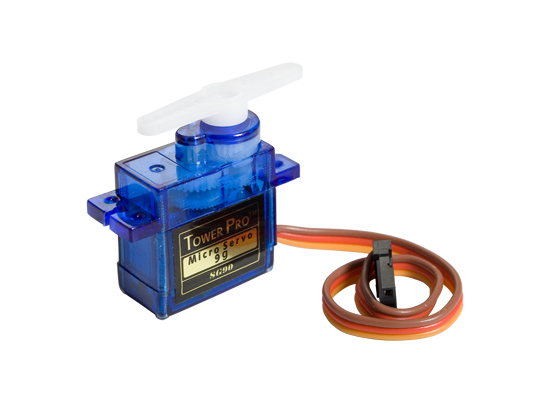
\includegraphics[width=0.4\textwidth]{../Files/tower-pro-sg90.jpg}
	\caption{Micro-Servo Motor}  \label{fig:Servo}
\end{figure}
We had to use a servo motor in order to rotate the \hcsr{} and give it a wider field of view over the area around it. This \servo{} can rotate approximately 180 degrees(90 in each side) with an operating speed of 0.1s/60degrees. Moreover, it has an operating voltage of 4.8V(~5V) which is in the same range as of the \arduinouno{}.\\
Other details:
\begin{itemize}
	\item Weight: 9 g
	\item Dimension: 22.2 x 11.8 x 31 mm approx.
	\item Stall torque: 1.8 kgf·cm
	\item Operating speed: 0.1 s/60 degrees
	\item Operating voltage: 4.8 V (~5V)
	\item Deadband width: 10 us (The servo will not move so long as subsequent commands to it are within the deadband timing pulse width)
	\item Temperature range: 0-55C
\end{itemize}
The \servo{} has a \emph{signal} pin to which the arduino sends the value of angle that it should turn to. Figure \ref{fig:pinServo} shows the pins of the \servo{}.
\begin{figure}[H]
	\centering
	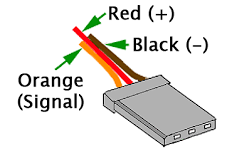
\includegraphics[width=0.4\textwidth]{../Files/microservo.png}
	\caption{Pins of Micro-Servo}  \label{fig:pinServo}
\end{figure}
The \ultrasonic{} was mounted on top of it and the apparatus connected to the arduino was kept in a modified transparent plastic case, as shown in Figure \ref{fig:projphoto}.
\begin{figure}[H]
	\centering
	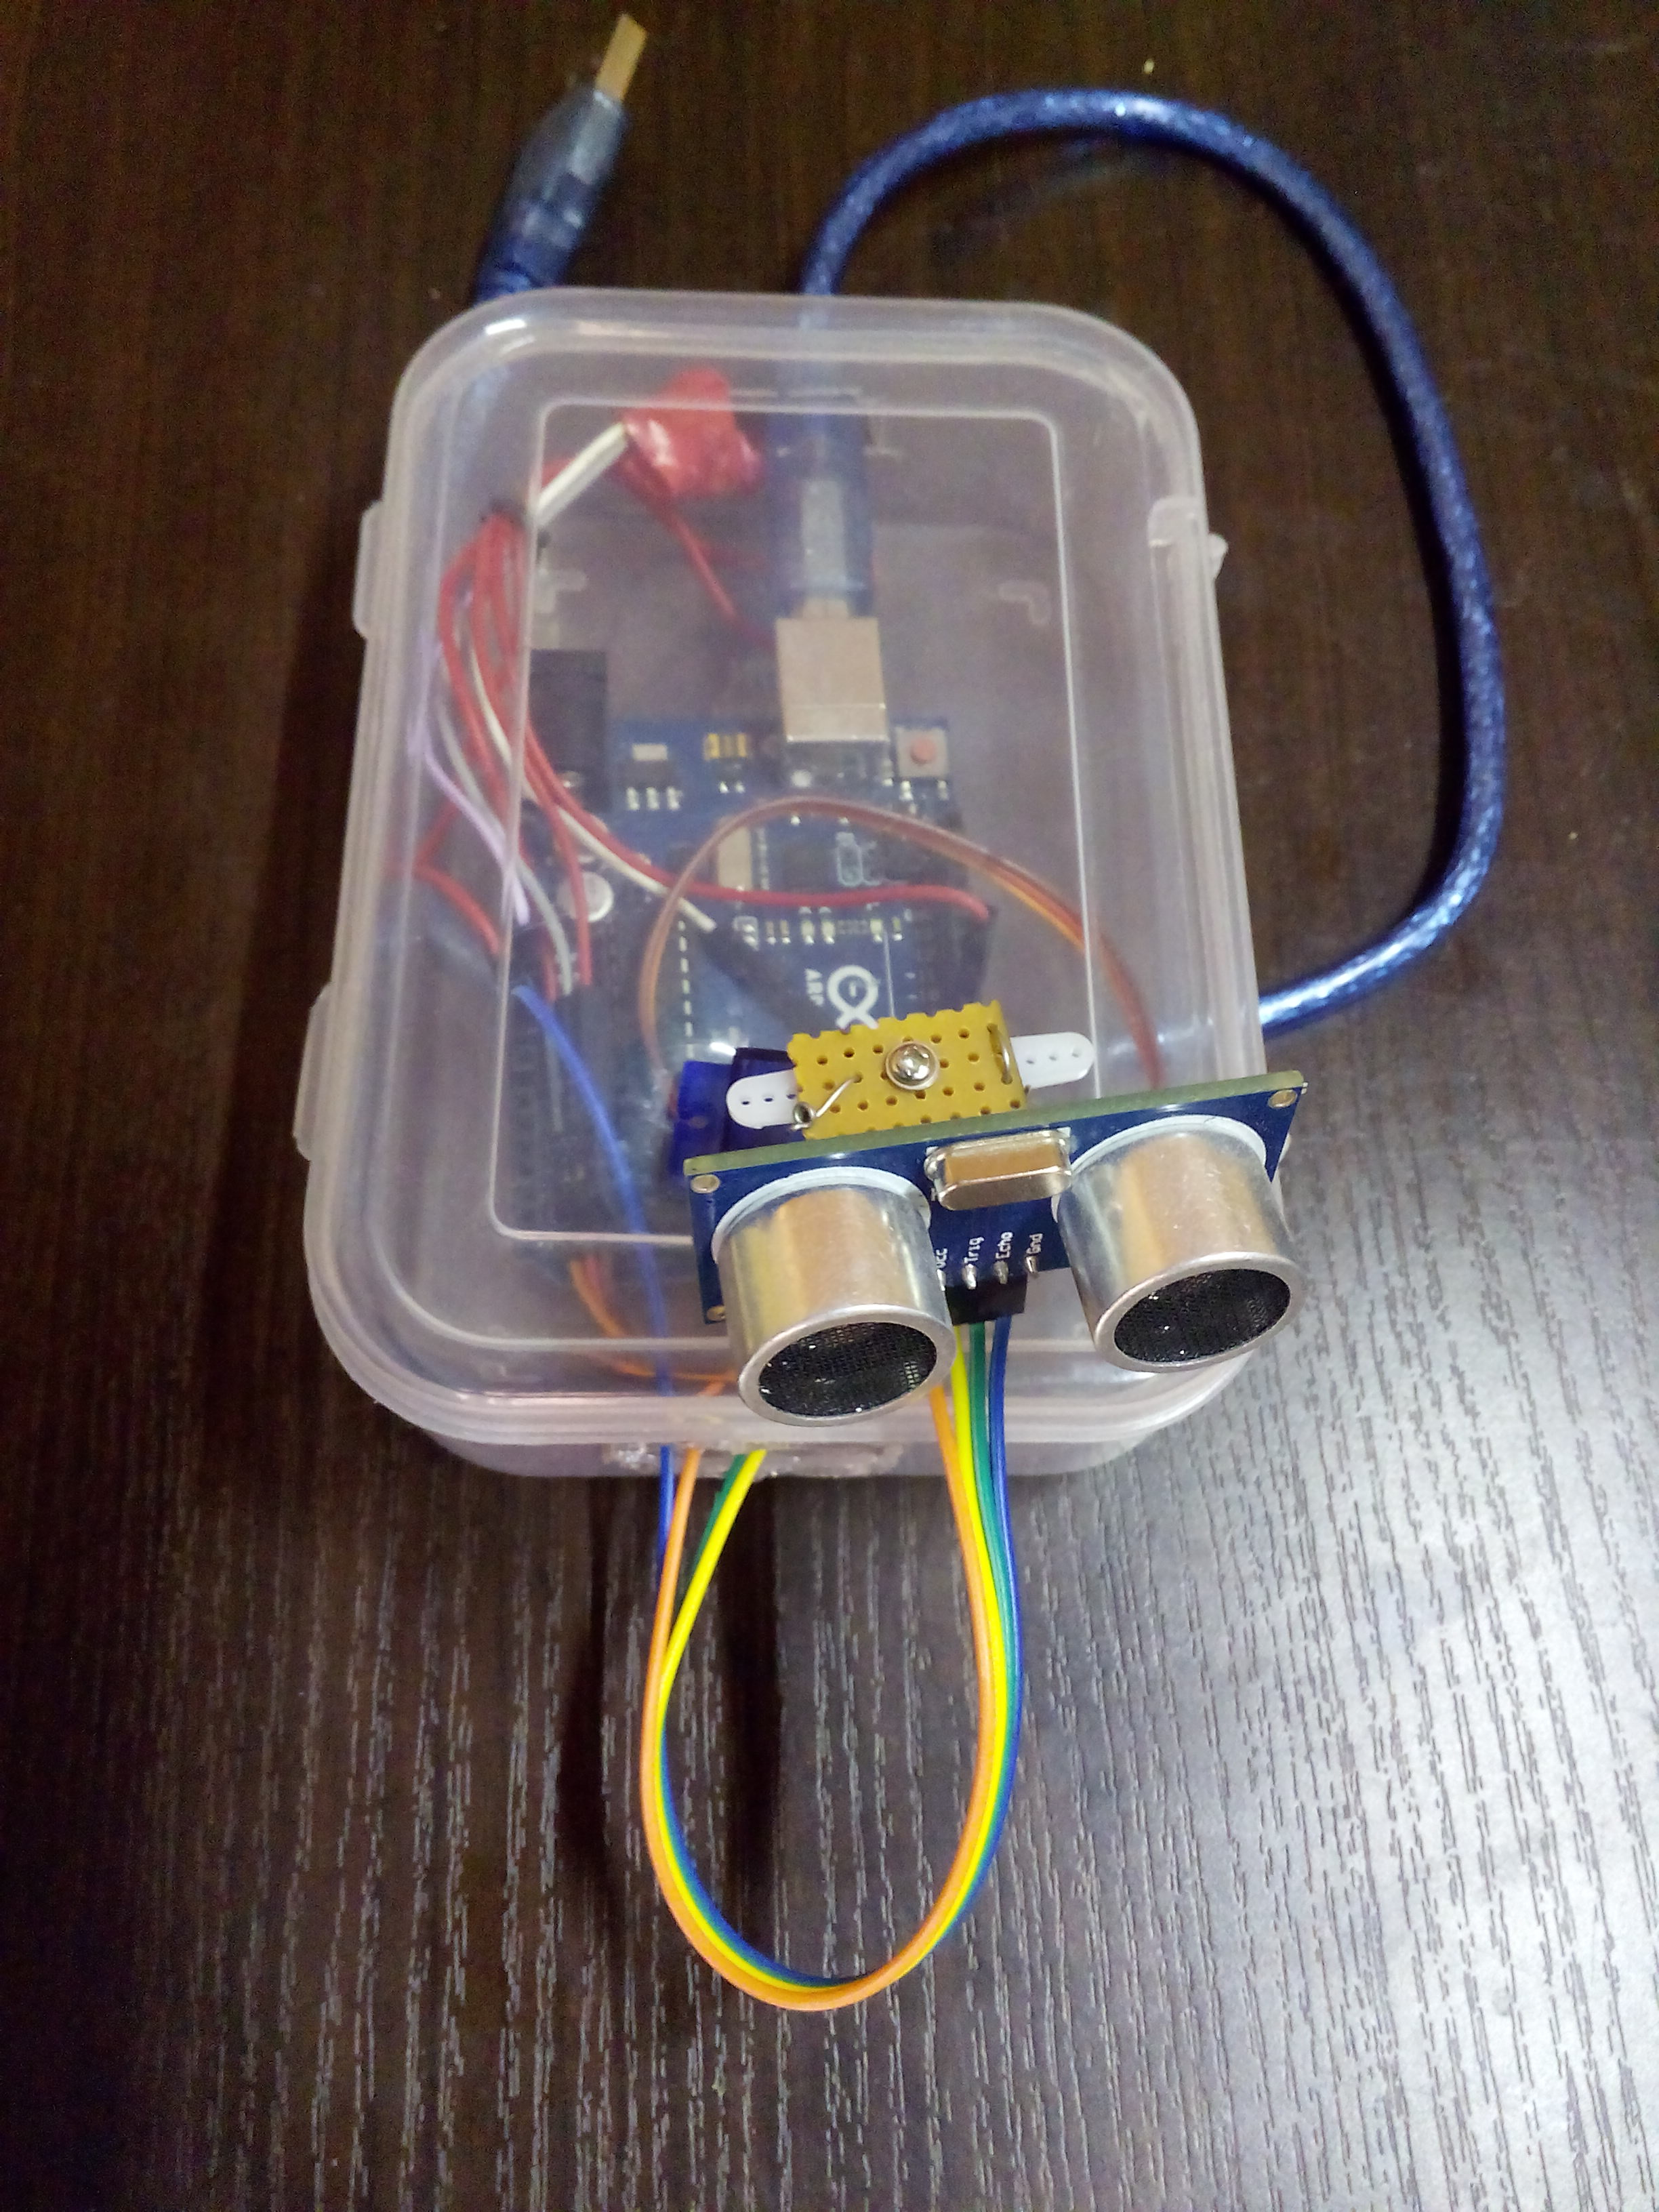
\includegraphics[width=0.4\textwidth]{../Files/proj.jpg}
	\caption{The Apparatus}  \label{fig:projphoto}
\end{figure}
We then proceeded to deciding the circuit connections, as shown in the next section.
\clearpage